% PRL look and style (easy on the eyes)
\documentclass[aps,pre,twocolumn,nofootinbib,superscriptaddress,linenumbers,11point]{revtex4-1}
% Two-column style (for submission/review/editing)
%\documentclass[aps,prl,preprint,nofootinbib,superscriptaddress,linenumbers]{revtex4-1}

%\usepackage{palatino}

% Change to a sans serif font.
\usepackage{sourcesanspro}
\renewcommand*\familydefault{\sfdefault} %% Only if the base font of the document is to be sans serif
\usepackage[T1]{fontenc}
%\usepackage[font=sf,justification=justified]{caption}
\usepackage[font=sf]{floatrow}

% Rework captions to use sans serif font.
\makeatletter
\renewcommand\@make@capt@title[2]{%
 \@ifx@empty\float@link{\@firstofone}{\expandafter\href\expandafter{\float@link}}%
  {\textbf{#1}}\sf\@caption@fignum@sep#2\quad
}%
\makeatother

\usepackage{amsmath}
\usepackage{amssymb}
\usepackage{graphicx}
%\usepackage[mathbf,mathcal]{euler}
%\usepackage{citesort}
\usepackage{dcolumn}
\usepackage{boxedminipage}
\usepackage{verbatim}
\usepackage[colorlinks=true,citecolor=blue,linkcolor=blue]{hyperref}


% The figures are in a figures/ subdirectory.
\graphicspath{{figures/}}

% italicized boldface for math (e.g. vectors)
\newcommand{\bfv}[1]{{\mbox{\boldmath{$#1$}}}}
% non-italicized boldface for math (e.g. matrices)
\newcommand{\bfm}[1]{{\bf #1}}          

%\newcommand{\bfm}[1]{{\mbox{\boldmath{$#1$}}}}
%\newcommand{\bfm}[1]{{\bf #1}}
\newcommand{\expect}[1]{\left \langle #1 \right \rangle}                % <.> for denoting expectations over realizations of an experiment or thermal averages

% vectors
\newcommand{\x}{\bfv{x}}
\newcommand{\y}{\bfv{y}}
\newcommand{\f}{\bfv{f}}

\newcommand{\bfc}{\bfm{c}}
\newcommand{\hatf}{\hat{f}}

\newcommand{\bTheta}{\bfm{\Theta}}
\newcommand{\btheta}{\bfm{\theta}}
\newcommand{\bhatf}{\bfm{\hat{f}}}
\newcommand{\Cov}[1] {\mathrm{cov}\left( #1 \right)}
\newcommand{\Ept}[1] {{\mathrm E}\left[ #1 \right]}
\newcommand{\Eptk}[2] {{\mathrm E}\left[ #2 \,|\, #1\right]}
\newcommand{\T}{\mathrm{T}}                                % T used in matrix transpose
\newcommand{\conc}[1] {\left[ \mathrm{#1} \right]}

\newcommand{\pyitc}{\url{http://www.simtk.org/home/bayesian-itc}} % URL of pyITC project homepage

%%%%%%%%%%%%%%%%%%%%%%%%%%%%%%%%%%%%%%%%%%%%%%%%%%%%%%%%%%%%%%%%%%%%%%%%%%%%%%%%
% DOCUMENT
%%%%%%%%%%%%%%%%%%%%%%%%%%%%%%%%%%%%%%%%%%%%%%%%%%%%%%%%%%%%%%%%%%%%%%%%%%%%%%%%

\begin{document}

%%%%%%%%%%%%%%%%%%%%%%%%%%%%%%%%%%%%%%%%%%%%%%%%%%%%%%%%%%%%%%%%%%%%%%%%%%%%%%%%
% TITLE
%%%%%%%%%%%%%%%%%%%%%%%%%%%%%%%%%%%%%%%%%%%%%%%%%%%%%%%%%%%%%%%%%%%%%%%%%%%%%%%%

\title{A simple method for automated equilibration detection in molecular simulations}

\author{John D. Chodera}
 \thanks{Corresponding author}
 \email{john.chodera@choderalab.org}
 \affiliation{Computational Biology Program, Sloan Kettering Institute, Memorial Sloan Kettering Cancer Center, New York, NY 10065}

\date{\today}

%%%%%%%%%%%%%%%%%%%%%%%%%%%%%%%%%%%%%%%%%%%%%%%%%%%%%%%%%%%%%%%%%%%%%%%%%%%%%%%%
% ABSTRACT
%%%%%%%%%%%%%%%%%%%%%%%%%%%%%%%%%%%%%%%%%%%%%%%%%%%%%%%%%%%%%%%%%%%%%%%%%%%%%%%%

\begin{abstract}

Molecular simulations intended to compute equilibrium properties (such as molecular dynamics and Metropolis Monte Carlo simulations) are often initiated from configurations that are highly atypical of equilibrium samples, a practice which typically generates a distinct initial transient in mechanical observables computed over the timecourse of the simulation.
Traditional practice in simulation data analysis recommends this initial transient portion be discarded to \emph{equilibration}, but no simple, general, and automated procedure for this process exists.
Here, we consider a conceptually simple, automated, easy-to-implement procedure that does not make strict assumptions about the distribution of the observable of interest, in which the equilibration region is chosen to maximize the number of effectively uncorrelated samples in the production portion used for computing equilibrium averages.
We present a simple reference Python implementation of this procedure and illustrate its application to both synthetic and real simulation data.\\

% KEYWORDS
\emph{Keywords: molecular dynamics (MD); Monte Carlo (MC); Markov chain Monte Carlo (MCMC); equilibration; timeseries analysis; statistical inefficiency; integrated autocorrelation time}

\end{abstract}

\maketitle

%%%%%%%%%%%%%%%%%%%%%%%%%%%%%%%%%%%%%%%%%%%%%%%%%%%%%%%%%%%%%%%%%%%%%%%%%%%%%%%%
% INTRODUCTION
%%%%%%%%%%%%%%%%%%%%%%%%%%%%%%%%%%%%%%%%%%%%%%%%%%%%%%%%%%%%%%%%%%%%%%%%%%%%%%%%

\section*{Introduction}
\label{section:introduction}

Molecular simulations use Markov chain Monte Carlo (MCMC) techniques~\cite{jun-s-liu:mcmc} to sample configurations $x$ from an equilibrium distribution $\pi(x)$, either exactly (using Monte Carlo methods) or approximately (using molecular dynamics simulations without Metropolization)~\cite{sivak:2013:prx:vvvr}.

Due to the sensitivity of the equilibrium distribution $\pi(x)$ to small perturbations in configuration $x$ and the difficulty of producing sufficiently good guesses of typical equilibrium configurations, these molecular simulations are often started from highly atypical initial conditions.
For example, simulations of biopolymers might be initiated from a fully extended conformation unrepresentative of behavior in solution, or a geometry derived from a fit to diffraction data collected from a cryocooled crystal; 
solvated systems may be prepared by periodically replicating a small solvent box equilibrated under different conditions, yielding atypical densities; 
liquid mixtures or lipid bilayers may be constructed by using methods that fulfill spatial constraints but create locally aytpical geometries (e.g.~PackMol~\cite{martinez:jctc:2009:packmol}), requiring long simulation times to relax to typical configurations.

As a result, traditional practice in molecular simulation has been to discard some initial portion of the trajectory to ``equilibration'' (also called \emph{burn-in}\footnote{The term \emph{burn-in} comes from the field of electronics, in which a short ``burn-in'' period is used to ensure that a device is free of faulty components---which often fail quickly---and is operating normally~\cite{crc-mcmc-handbook}.} in MCMC literature~\cite{crc-mcmc-handbook}).
While this practice is strictly unnecessary for the time-average of quantities of interest to converge to the desired expectations~\cite{geyer:burn-in-unnecessary,crc-mcmc-handbook}, this process often allows the practitioner to avoid impractically long run times to eliminate the bias in computed properties in finite-length simulations induced by atypical initial starting conditions.

% Liquid argon example
% JDC: Should we use TIP3P water instead?
As an illustrative example, consider the simulation shown in {Figure~\ref{figure:burn-in-example}}, in which a simulation of liquid argon is started at an atypical density and allowed to relax to its equilibrium density ({Figure~\ref{figure:burn-in-example}, top}).
The expectation of the running average of the density over many realizations of this procedure ({Figure~\ref{figure:burn-in-example}, bottom}) significantly deviates from the actual expectation, which would lead to biased estimates unless simulations were sufficiently long to eliminate this starting point dependent bias.
Note that this significant bias is present because the \emph{same} atypical starting condition is used for every realization of this simulation process.

For the purposes of this note, we presume that the goal is to compute some form of equilibrium expectation, $\expect{A}$ from a timeseries average:

Consider successively sampled configurations $x_t$, $t = 1, \ldots, T$ from a molecular simulation.
We presume we are interested in the expectation $\expect{A} \equiv \int dx \, A(x) \, \pi(x)$ of a mechanical property $A(x)$.
For convenience, we will refer to the timeseries $A_t \equiv A(x_t)$, with $t = 0$.
The estimator $\hat{A} \approx \expect{A}$ constructed from the entire dataset is given by
\begin{eqnarray}
\hat{A}_{[1,T]} \equiv \frac{1}{T} \sum_{t=1}^T A_t . \label{equation:time-average}
\end{eqnarray}
While $\lim_{T \rightarrow \infty} \hat{A}_{[1,T]} = \expect{A}$\footnote{We note that this equality only holds for simulation schemes that sample from the true equilibrium distribution $\pi(x)$, such as Metropolis-Hastings Monte Carlo or Metropolized integration schemes. Molecular dynamics simulations utilizing finite timestep integration without Metropolization will produce averages that may deviate from the true expectation $\expect{A}$~\cite{deviation}.}, we concern ourselves here with the optimal approach to estimating $\expect{A}$ given a simulation of \emph{finite} time $T$.

%%%%%%%%%%%%%%%%%%%%%%%%%%%%%%%%%%%%%%%%%%%%%%%%%%%%%%%%%%%%%%%%%%%%%%%%%%%%%%%%
% FIGURE: BURN-IN EXAMPLE
%%%%%%%%%%%%%%%%%%%%%%%%%%%%%%%%%%%%%%%%%%%%%%%%%%%%%%%%%%%%%%%%%%%%%%%%%%%%%%%%

\begin{figure*} 
\resizebox{0.9\textwidth}{!}{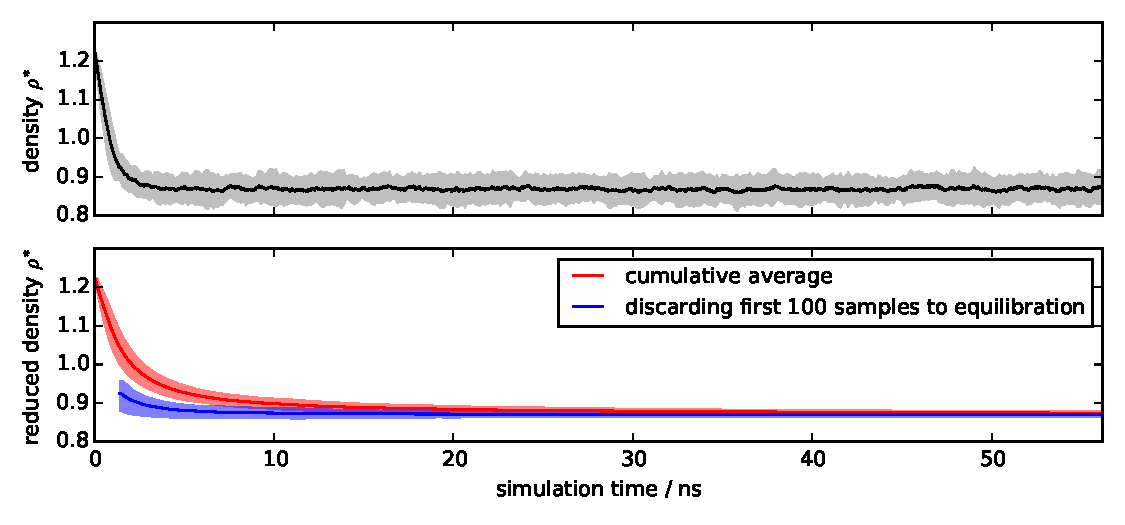
\includegraphics{argon-density.pdf}}
\caption{\label{figure:burn-in-example} {\bf Illustration of the motivation for discarding data to equilibration.} 
To illustrate the bias in expectations induced by relaxation away from initial conditions, 100 replicates of a simulation of liquid argon were initiated from the same energy-minimized initial configuration constructed with initial reduced density $\rho^* \equiv \rho \sigma^3 = 0.960$ but different random number seeds for stochastic integration.
%
{\bf Top:} The average of the reduced density (black line) over the replicates relaxes to the region of typical equilibrium densities over the first few ns of simulation time.
%
{\bf Bottom:} If the average density is estimated by a cumulative average from the beginning of the simulation (red line), the estimate will be heavily biased by the atypical starting density even beyond 10 ns.
Discarding even a small amount of initial data---in this case 100 initial samples (blue line)---results in a cumulative average estimate that converges to the true average (black dotted line) much more rapidly.
% 
Shaded regions denote 95\% confidence intervals.
%
Simulations were performed using a box of $N = 500$ argon atoms at reduced temperature $T^* \equiv k_B T / \epsilon = 0.850$ and reduced pressure $p^* \equiv p \sigma^3 / \epsilon = 1.266$ using a Langevin integrator~\cite{sivak-chodera-crooks:jpcb:2014:vvvr} with timestep $\Delta t = 0.01 \tau$, where characteristic oscillation timescale $\tau = \sqrt{m r_0^2 / 72 \epsilon}$, with $r_0 = 2^{1/6} \sigma$~\cite{liquid-argon-characteristic-timescale}.
A Metropolis Monte Carlo barostat was used with box volume moves attempted every 25 timesteps.
Densities were recorded every 25 timesteps.
}
\end{figure*}

%%%%%%%%%%%%%%%%%%%%%%%%%%%%%%%%%%%%%%%%%%%%%%%%%%%%%%%%%%%%%%%%%%%%%%%%%%%%%%%%
% STATISTICAL INEFFICIENCY
%%%%%%%%%%%%%%%%%%%%%%%%%%%%%%%%%%%%%%%%%%%%%%%%%%%%%%%%%%%%%%%%%%%%%%%%%%%%%%%%

\section*{Effective number of uncorrelated samples}
\label{section:statistical-inefficiency}

An important concept in the development of the main idea presented here is the notion of the \emph{effective number of uncorrelated samples} present in a sample of correlated timeseries data and the related concept of \emph{statistical inefficiency}.
While this is well-established for the analysis of both Monte Carlo and molecular dynamics simulations~\cite{}, we review it here for the sake of clarity.

We first 

%%%%%%%%%%%%%%%%%%%%%%%%%%%%%%%%%%%%%%%%%%%%%%%%%%%%%%%%%%%%%%%%%%%%%%%%%%%%%%%%
% THE IDEA
%%%%%%%%%%%%%%%%%%%%%%%%%%%%%%%%%%%%%%%%%%%%%%%%%%%%%%%%%%%%%%%%%%%%%%%%%%%%%%%%

\section*{The idea}
\label{section:the-idea}

Suppose we choose some arbitrary time $t_0$ and discard all samples $t \in [0, t_0)$ to equilibration, keeping $[t_0, T]$ as the dataset to analyze.
How much data remains?
We can determine this by computing the statistical inefficiency $g_{t_0}$ for the interval $[t_0, T]$, and computing the effective number of uncorrelated samples $N_\mathrm{eff}(t_0) \equiv (T - t_0 + 1) / g_{t_0}$.
If we start at $t_0 \equiv T$ and move $t_0$ to earlier and earlier points in time, we expect that the effective number of uncorrelated samples $N_\mathrm{eff}(t_0)$ will continue to grow until we start to include the highly atypical initial data.
At that point, the integrated autocorrelation time $\tau$ (and hence the statistical inefficiency $g$) will greatly increase, and the effective number of samples $N_\mathrm{eff}$ will start to plummet.


%%%%%%%%%%%%%%%%%%%%%%%%%%%%%%%%%%%%%%%%%%%%%%%%%%%%%%%%%%%%%%%%%%%%%%%%%%%%%%%%
% METHODS
%%%%%%%%%%%%%%%%%%%%%%%%%%%%%%%%%%%%%%%%%%%%%%%%%%%%%%%%%%%%%%%%%%%%%%%%%%%%%%%%

\section*{Illustration}
\label{section:methods}

All molecular simulations were performed with OpenMM 6.2~\cite{eastman:jctc:2012:openmm} using the Python API.
All scripts used to run simulations, analyze data, and generate plots---along with the simulation data itself---are availabile on GitHub at \url{http://github.com/choderalab/automatic-equilibration-detection}.

%%%%%%%%%%%%%%%%%%%%%%%%%%%%%%%%%%%%%%%%%%%%%%%%%%%%%%%%%%%%%%%%%%%%%%%%%%%%%%%%
% ACKNOWLEDGMENTS
%%%%%%%%%%%%%%%%%%%%%%%%%%%%%%%%%%%%%%%%%%%%%%%%%%%%%%%%%%%%%%%%%%%%%%%%%%%%%%%%

\section*{Acknowledgments}

We are grateful to William C.~Swope (IBM Almaden Research Center), Kyle A.~Beauchamp (MSKCC), and Robert C.~McGibbon (Stanford University) for valuable discussions on this topic, and Joshua L.~Adelman (University of Pittsburgh) for helpful feedback and encouragement.

%%%%%%%%%%%%%%%%%%%%%%%%%%%%%%%%%%%%%%%%%%%%%%%%%%%%%%%%%%%%%%%%%%%%%%%%%%%%%%%%
% BIBLIOGRAPHY
%%%%%%%%%%%%%%%%%%%%%%%%%%%%%%%%%%%%%%%%%%%%%%%%%%%%%%%%%%%%%%%%%%%%%%%%%%%%%%%%

\bibliographystyle{prsty} 
\bibliography{automatic-equilibration-detection}

\end{document}